\chapter{Simulation Results}
\label{sec:results}

In the following, the results of the thesis will be discussed.
The performance of the optimization routine will be shown for different settings, i.e. for different number of relays, receiving antennas per user, users, relay placings, and input powers.
If not any further mentioned, the same settings will be used, as in Section~\ref{sec:solver}, i.e.
we will look at a two user system with one receive antenna and three relays per user, as shown in Figure~\ref{fig:antenna_placing}.
The relays in this system will be lossless, i.e. the impedance will be pure imaginary.
Additionally only s noise contribution of the circuitry after the LNA, i.e. only downstream noise (c.f. Equation~\eqref{eq:noise_contrib}) will be considered.
Therefore, because of the unilateral assumption, the noise contribution will be i.i.d. and independent of the matching network or the relays.
Hence, the optimization algorithm is only able to adapt the signal and the interference.

\section{Introduction of Measures for Comparison}
\label{sec:measures}
To be able to rate the results on how good they are, the performance will be compared to classical interference eliminating methods such as TDMA.
Additionally, improvements from the uncoupled case will be given, as well as theoretical performance limits in order to see by how much the performance can be pushed.
In the following, the rates, to which the optimization is compared to will be introduced.
\begin{figure}[h]
\centering
  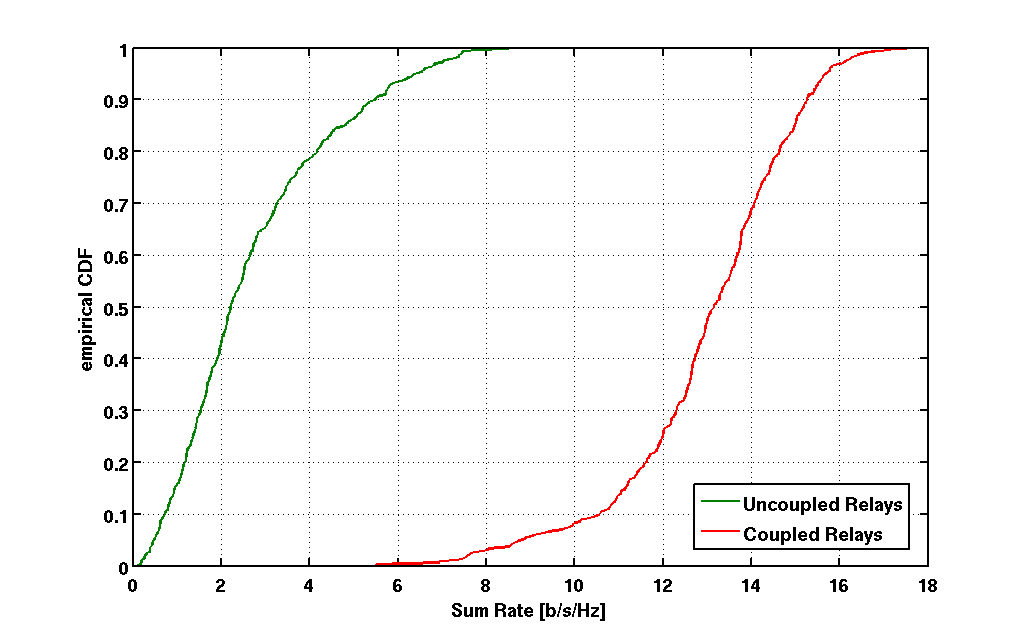
\includegraphics[width=0.85\linewidth]{images/Coupledcomparison.png}
\caption{Comparison of uncoupled relays and optimized coupled relays.}
\label{fig:coupledcomparison}
\end{figure}

\subsection{Uncoupled Relay Rates}
One of the logical performances to compare the use of loaded antennas to, is the same setting without any coupling among the relays.
Logically, the "uncoupled relays rate" should be smaller than including the relays and adapting their impedances to our needs.
If no higher rate can be achieved, the whole idea of using passive relays would fail.


In Figure~\ref{fig:coupledcomparison}, the green solid line shows the performance if no coupling among the relays and receivers exist.
It is clear, that the rates including relay coupling (red solid line) are much larger.
Therefore this method is suitable to improve the achievable rates.


\subsection{TDMA Rates}
The next performance, the optimized rates are compared to are the TDMA rates for the equivalent setup.
Therefore, the relays are again assumed to be uncoupled from the receivers and the transmit/receive pairs are assumed to divide the time equally among each other for transmission.
For the calculation the formulas from Equation~\eqref{eq:tdma_achiev_rate} and~\eqref{eq:tdma_achiev_sum_rate} are used.

\begin{figure}[h]
\centering
  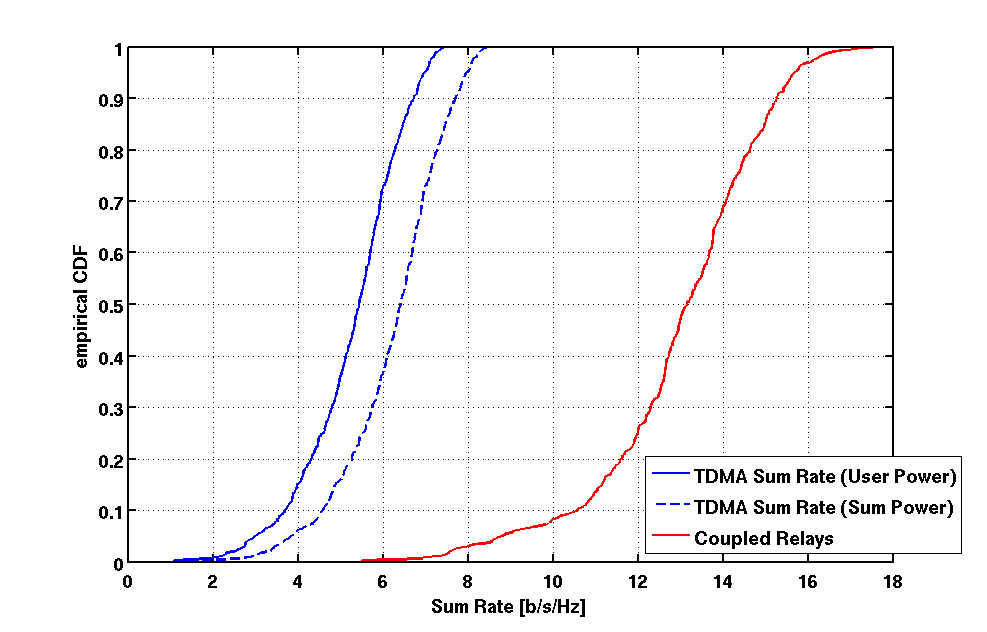
\includegraphics[width=0.9\linewidth]{images/TDMAcomparison.png}
\caption{Comparison of the TDMA rate and optimized coupled relays.}
\label{fig:TDMAcomparison}
\end{figure}

In Figure~\ref{fig:TDMAcomparison}, the blue solid line shows the performance if TDMA was applied under the user-power constraint (i.e. the limit of the transmit power is given per user and therefore the same for each user as in the coupled relay case) and the relays were uncoupled from the receivers.
The blue dashed line shows the performance of TDMA under the sum power constraint (i.e. the limit of the transmit power is given by the total transmit power and therefore the power per user in TDMA is $N_\text{User}$ times the power per user in the coupled relay case - here two times).
As before, the rates including relay coupling (red solid line) are much larger than without any coupling and TDMA.
Of course this comparison is more dependent on the choice of the settings (especially the choice of the number of transmit-receive pairs) and we will see different behaviors in the following sections. 

\subsection{Noise-free Rates}
\label{sec:sir}
As we are addressing the problem of interference, a good measure is the noise-free rate (short: SIR-rate).
It is calculated similar to the SINR-rate, however it only considers the interference and not the noise (c.f. Equation~\eqref{eq:sir_rate}).
As written in the previous chapters, in high SNR regime, the interference is the main diminishing factor for the rates (c.f. Section~\ref{sec:rates}), the SIR-rates will give an indicator, on how good the relays and the matching network were optimized.
Example curves of the SIR-rates (blue dashed lines) can be seen in Figures~\ref{fig:relcomp_1}~to~\ref{fig:relcomp_3}.

\subsection{Relays as Fully Cooperation Receivers - Limit}
\label{sec:fullrx_limit}
The remaining two function to which the rates after the optimization algorithms are compared against will give limits on how good the method of loaded antennas can be at best.
The first approach is to see the relays as fully cooperation receivers, which are widely spread.
Hence they experience no coupling among each other.
The number of observations the receiver has on the incoming signals is increased to $N_\text{Rx} + N_\text{Relays}$.
As we choose the number of relays larger than the number of interferer in most of the cases, this method will lead to an interference free connection.

The performance of the fully cooperation relays can be seen in Figure~\ref{fig:limcomparison} (black solid curve).
At median it is almost $2 \left[\text{b/s/Hz}\right]$ higher, than the optimized rate of the passive coupled relays.
For the best 10\% of the cases this is reduced to $1 \left[\text{b/s/Hz}\right]$ and less,
for the worst 10\% of the cases this lies in between  $2.5 \left[\text{b/s/Hz}\right]$ and $4.7 \left[\text{b/s/Hz}\right]$.


\subsection{Multiport Matching - Limit}
\label{sec:mp_limit}
It has been shown that the multiport matching is the optimal setting for a matching network (without considering any coupling among the receivers, and any relays)~\cite{Nossek}.
For the comparison with the coupled relays, the relays are, as in the previous section, assumed to be fully cooperating receiver antennas.
\begin{figure}[h]
\centering
  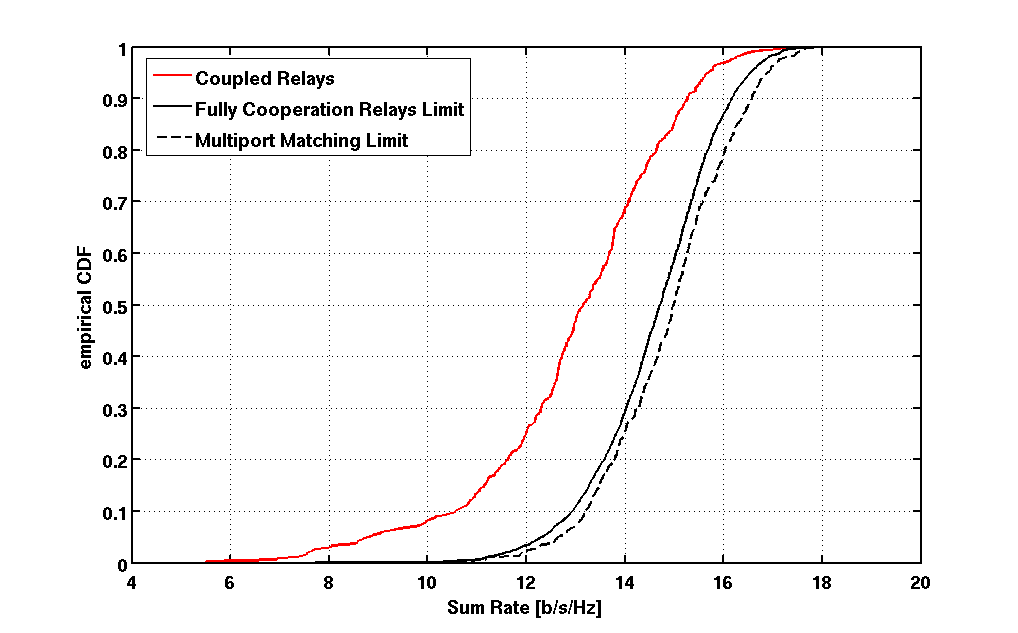
\includegraphics[width=0.9\linewidth]{images/Limitcomparison.png}
\caption{Comparison of the full cooperation relay rates, the multiport matching rate and optimized coupled relays rate.}
\label{fig:limcomparison}
\end{figure}
However, the placing of the relays remains the same, i.e. no widely spread receivers are assumed.
The number of observations one receiver has, is again $N_\text{Rx} + N_\text{Relays}$.
And hence it can be expected, that it is higher than the optimized coupled relays rate.
In Figure~\ref{fig:limcomparison} and the following, this limit is shown by the black dashed line.

\begin{figure}[h]
\centering
  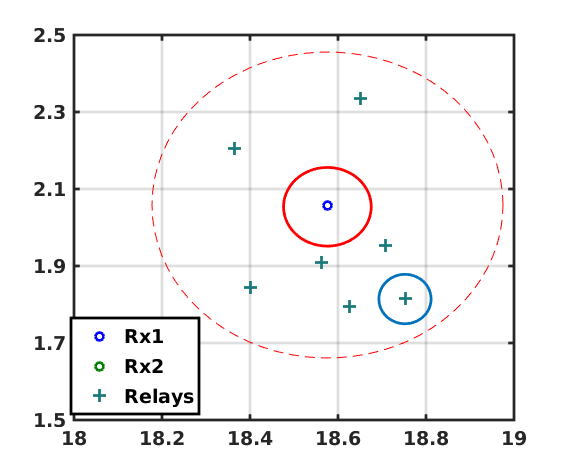
\includegraphics[width=0.6\linewidth]{images/cloud.png}
\caption{Placing the relays around a receiver uniformly distributed on a disk.}
\label{fig:cloud}
\end{figure}
\section{Relay Placing}
\label{sec:relay_placing}

Before analyzing the solver with different settings, the placing of the relays around a receiver is discussed a bit more in detail.
Figure~\ref{fig:cloud} shows, by which criteria, the relays were placed.

The red solid circle (with radius $d_\text{z}$) denotes a zone around the receiver, in which no relays must not be placed.
The red dashed line shows the maximum distance at which the relays may be placed away from the receiver. 
Within those two lines, the relays are thrown uniformly distributed.
The blue circle (with radius $d_\text{Relay}$) around the relay at the right bottom denotes a zone in which no other relay may be placed, i.e. the minimum distance between each relay.
If there is a violation by the relay distances, all the relays are thrown again.
\begin{figure}[h]
\centering
  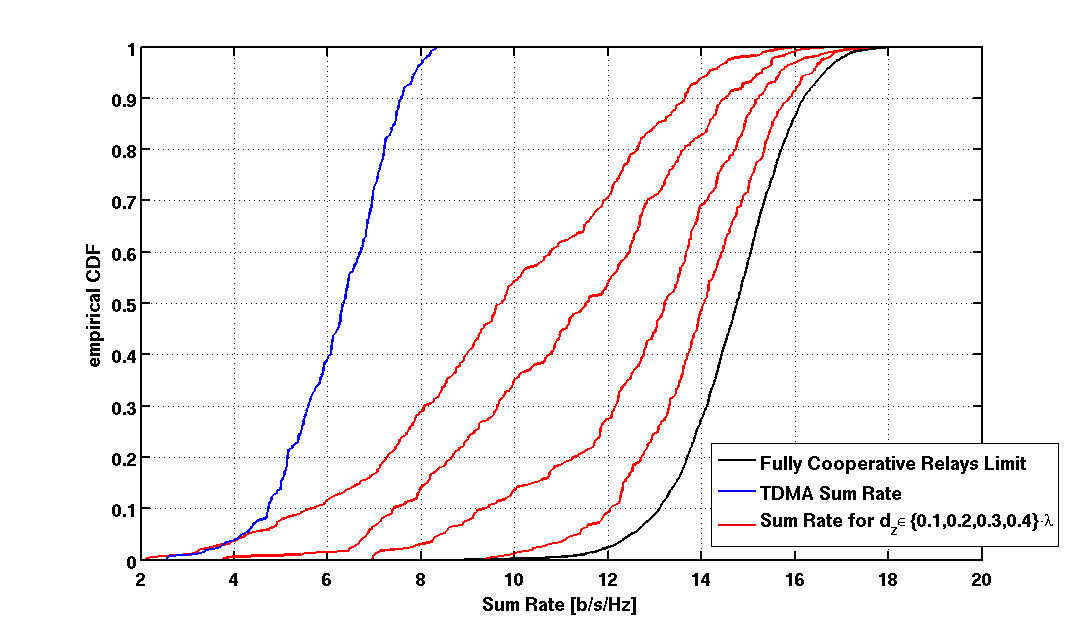
\includegraphics[width=0.8\linewidth]{images/Dzcomparison.png}
\caption{Optimized Sum Rates for different minimum distances between receiver and relays ($d_\text{z}\in\{0.1,0.2,0.3,0.4\}$ from right to left).}
\label{fig:dz_comparison}
\end{figure}

The minimum receiver distance and the minimum relay distance might differ, however, if not specially mentioned, they are assumed to be both $0.1\lambda$.
By a smaller choice of the maximum distance, the relays can be placed more dense.
When the maximum distance is set equal the minimum distance, the relays will be placed on a circle around the receiver.


Figure~\ref{fig:dz_comparison} shows the performance of the optimized sum rate for $d_\text{z}\in\{0.1,0.2,0.3,0.4\}\cdot\lambda$ (red curves from right to left).
For all the curves, the relays had the same minimum spacing, i.e. $d_\text{Relay}=0.1\cdot\lambda$.
Obviously a higher rate can be achieved, when the relays are closer to the receiver and thus the coupling is stronger.
Even with a minimum distance of 0.4$\lambda$, the achievable rate is higher than the the TDMA rate (blue solid curve) under the sum power constraint.

\section{Low SNR performance}
\label{sec:low_snr}

At first we want to analyze the optimization algorithm at different SNR levels.
Later we will only look at a high SNR level, as our aim is to minimize the interference.
As we assume only downstream noise, the optimization algorithm can only change the signal and the interference covariance matrices.
\begin{figure}[h]
\centering
  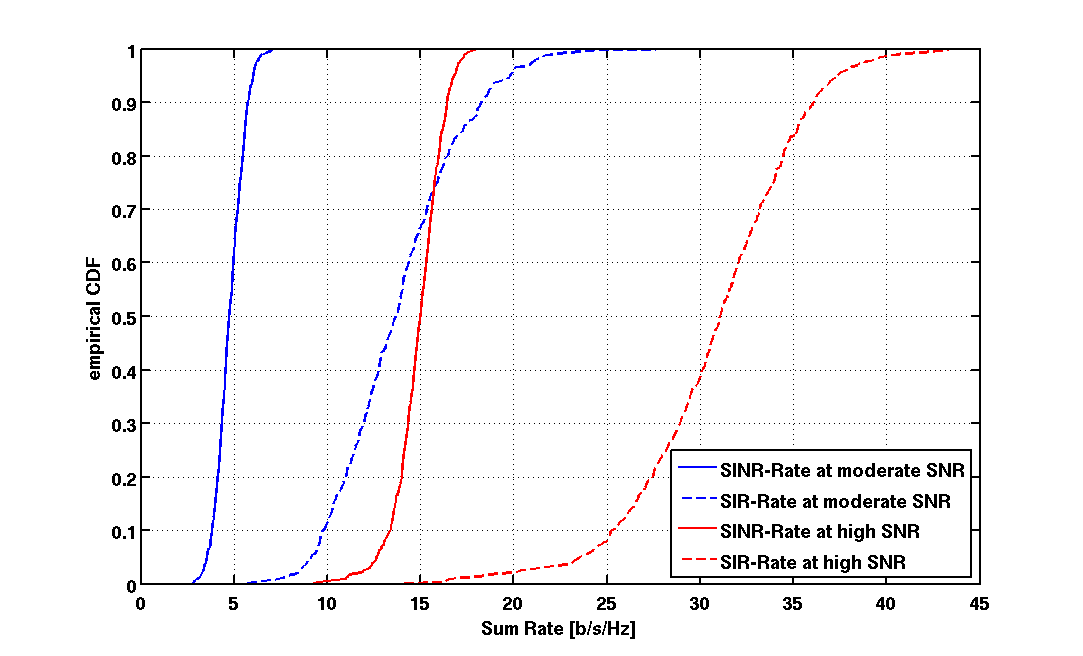
\includegraphics[width=0.9\linewidth]{images/Comparison_modvshighSNR.png}
\caption{Comparison of the optimization algorithm at a moderate and high SNR level and the comparison to the noise free (SIR) rates.}
\label{fig:snrcomparison}
\end{figure}

Figure~\ref{fig:snrcomparison} shows the SINR- and SIR- rates at a moderate SNR level (blue curves) and at a high SNR level (red curves).
As the achievable rate at a moderate SNR level (blue solid line) is less interference driven and more noise limited, the resulting SIR-rate (blue dashed curve) is also lower than the SIR-rate of the optimized achievable rate at a high SNR region (red dashed line).

This shows for the moderate SNR level, that the optimization algorithm was matching the values of the relays and the matching network in order to amplify the signal at first and only second reducing the interference.
For two users (as it is here the case) the interference is increased the same as the signal power (from moderate SNR to high SNR), hence if the optimization would have let to the same reduction of the interference at the moderate SNR level, the SIR rates would have become equivalent.

\section{Number of Relays to Eliminate Interference}
\label{sec:interf_fix}
In the following, the number of relays required for an interference free connections will be analyzed.
For the following plots, the number of receivers was set to one ($N_{R} = N_{R_x} = 1$) in order to increase the performance of the solver (c.f. Section~\ref{sec:stepwise}).

In the following sections the term "\textit{interference free}" will be used a couple of times.
Hereby only a reduced interference is meant.
Full interference elimination as in a MIMO system with more receive antennas than interferer will not be reached.
However when the term is used, the interference will be so low, that the effect of noise will be the same or even a stronger diminishing factor.

\subsection{One Interferer}
\label{sec:1interf}
To eliminate interference with two transmitters normally two observations are required.
Figure~\ref{fig:relcomp_1} shows the performance of a transmit/receiver pair with one interferer and $N_\text{Rel}\in\{1,2,3\}$ (red curves from left to right).
\begin{figure}[h]
\centering
  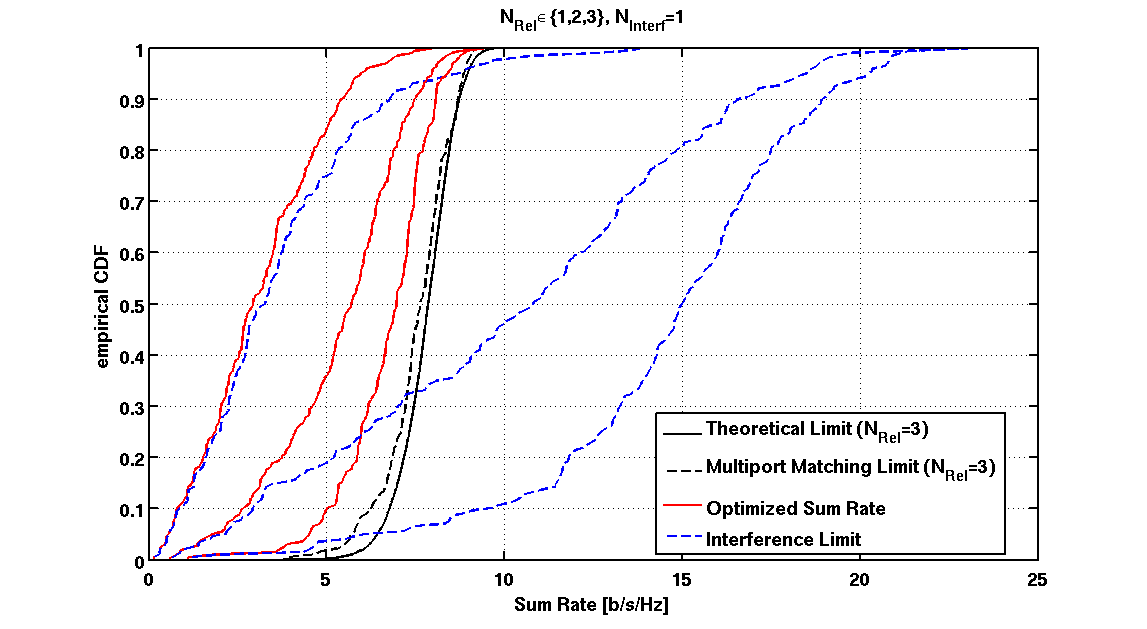
\includegraphics[width=0.9\linewidth]{images/Relcomparison_1interferer.png}
\caption{User rates for one interferer and one receiver with  $N_\text{Rel}\in\{1,2,3\}$ (red and blue curves from left to right) and their theoretical limits (black curves).}
\label{fig:relcomp_1}
\end{figure}
It is clear to see, that the higher the number of relays, the better the performance of the optimized system.
The blue dashed lines show the rates considering only the SI-ratio (c.f. Equation~\eqref{eq:sir_rate}).
The use of only one relay, leads only for 10\% of the cases to an interference free connection.
Increasing the number of relays to two leads to an interference free connection of almost 80\% of the realizations, however, to achieve for almost all realizations a noise limited connection at least three relays per receiver are required.

\begin{figure}[h]
\centering
  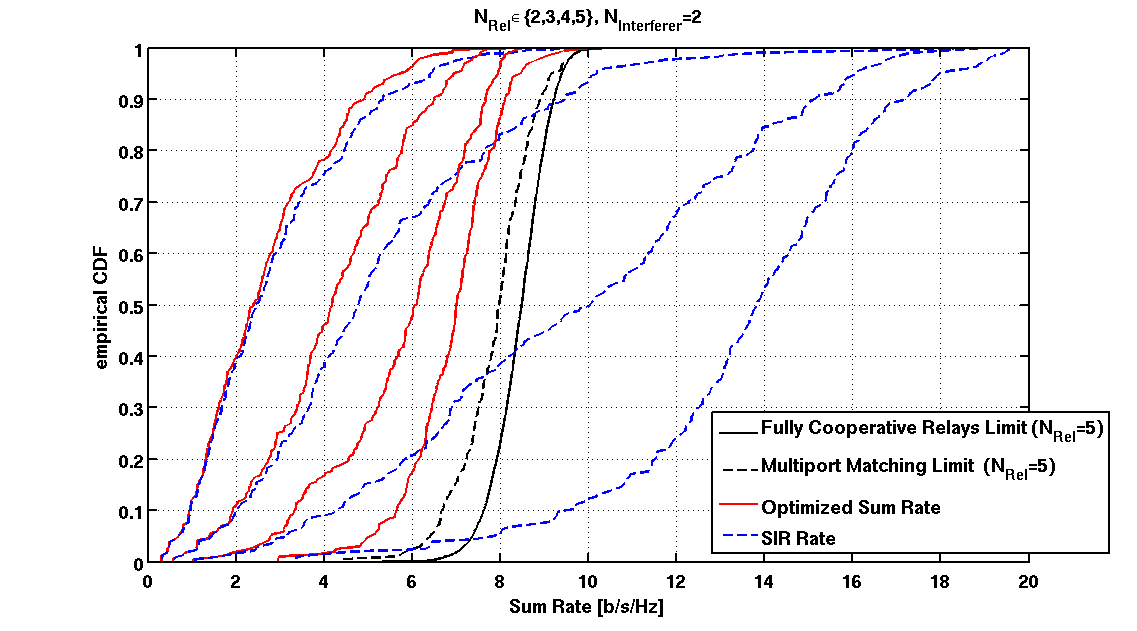
\includegraphics[width=0.9\linewidth]{images/Relcomparison_2interferer.png}
\caption{User rates for two interferer and one receiver with  $N_\text{Rel}\in\{2,3,4,5\}$ (red and blue curves from left to right) and their theoretical limits (black curves).}
\label{fig:relcomp_2}
\end{figure}
\subsection{Two Interferer}
\label{sec:2interf}
To eliminate interference with three transmitters normally three observations are required.
Figure~\ref{fig:relcomp_2} shows the performance of a transmit/receiver pair with two interferer and $N_\text{Rel}\in\{2,3,4,5\}$ (red curves from left to right).
And, as before, the blue dashed lines show the rates considering only the SI-ratio.

We see, that for two relays per user, the interference limited rate behaves almost the same as the optimized achievable user rate.
For three relays per user, some realizations lead to an interference free connection.
But only for five relays per user, over 90\% of the realizations can be driven into an low interference state.

\subsection{Three Interferer}
\label{sec:3interf}
To eliminate interference with four transmitters normally four observations are required.
Figure~\ref{fig:relcomp_3} shows the performance of a transmit/receiver pair with three interferer and $N_\text{Rel}\in\{4,5,6,7\}$ (red and blue dashed curves from left to right).
\begin{figure}[h]
\centering
  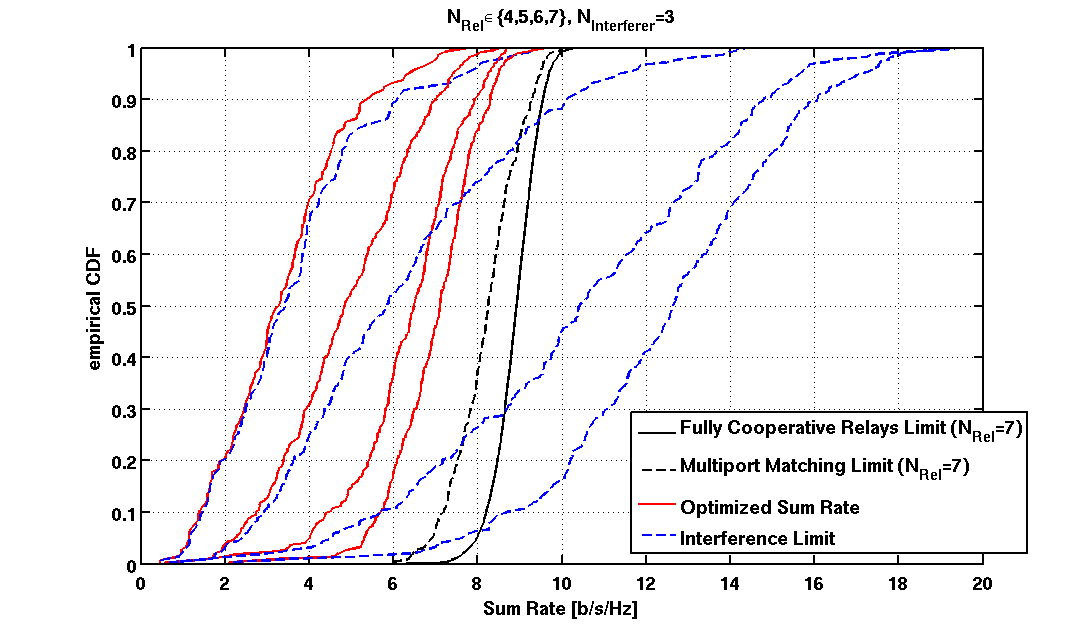
\includegraphics[width=0.9\linewidth]{images/Relcomparison_3interferer.png}
\caption{User rates for three interferer and one receiver with $N_\text{Rel}\in\{4,5,6,7\}$ (red and blue curves from left to right) and their theoretical limits (black curves).}
\label{fig:relcomp_3}
\end{figure}

We see, that for four relays per user, the interference limited rate behaves almost the same as the optimized achievable user rate.
For five and six relays per user, some realizations lead to an interference free connection.
For seven relays per user, over 90\% of the realizations can be driven into an low interference state.

Comparing this to the previous results with one and two interferer, we can see, that  the number of required relays to eliminate the interference grows not linearly as with the use of fully cooperating receivers.
It looks like, that it requires at least twice the number of interferer ($N_\text{Rel} > N_\text{Interferer}\cdot2$) per user, to overcome the interference.

\subsection{Cooperative versus Non-cooperative Receive Antennas}
\label{sec:rel_rx_comp}

In the following, we want to analyze what happens, if the number of relays plus receiver antennas is kept constant.
First, we analyze the case of one receive/transmit pair, as this decreases the size of the problem by a factor of four.
Behaviors as shown in Section~\ref{sec:stepwise} are therefore less likely to happen.
\begin{figure}[h]
\centering
  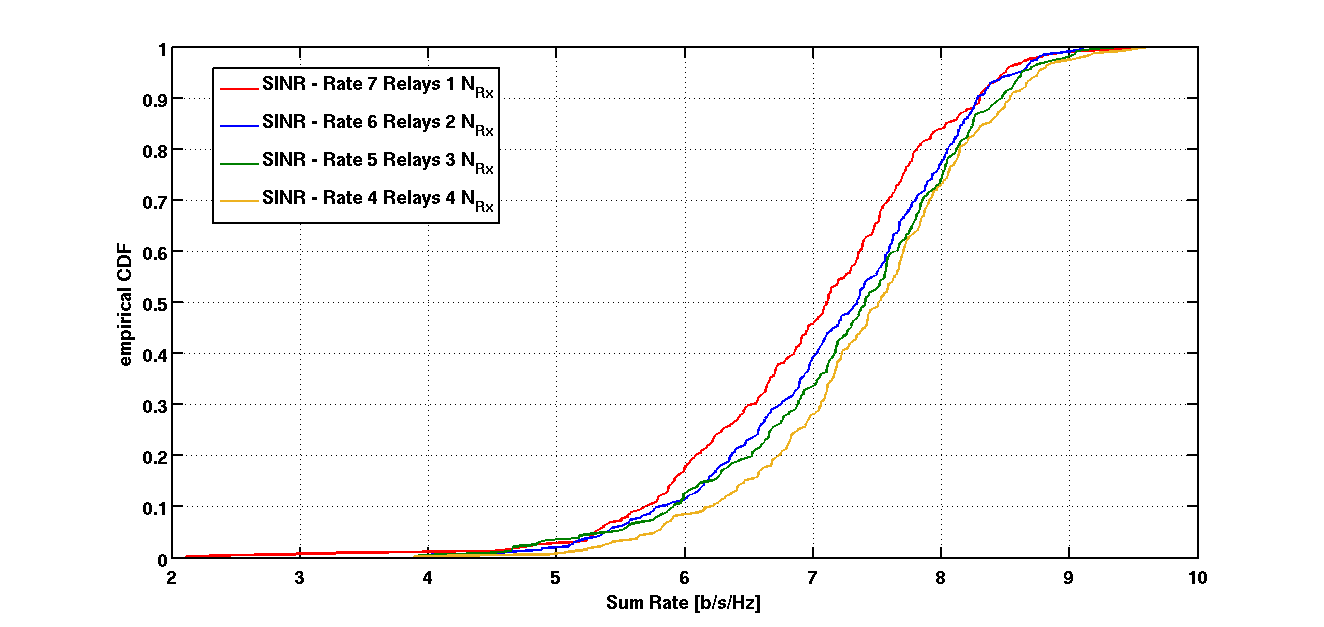
\includegraphics[width=\linewidth]{images/ConstNrelNrx8comparison_1Rx_onlySINR.png}
\caption{Comparison of constant $N_\text{Rel} + N_{\text{Rx}} = 8$, with $N_\text{Rel}\in\{4,5,6,7\}$ and $N_{\text{Rx}}\in\{1,2,3,4\}$ from left to right.}
\label{fig:1user_const}
\end{figure}
%\subsection{Constant Number of Receivers and Relays}
%\label{sec:1user_const}
Figure~\ref{fig:1user_const} shows the performance with three interferer and one transmit/receive pair.
Obviously in the case where four receive antennas were used (yellow curve), the interference can be fully zero forced therefore it also shows the highest rate.
However the performance is only $0.5 \left[\text{b/s/Hz}\right]$ smaller, if seven relays and only one receive antenna were used - for the values in between even less.
This shows, that with one additional observation and one relay less, the rate can not be improved significantly.
\begin{figure}[h]
\centering
  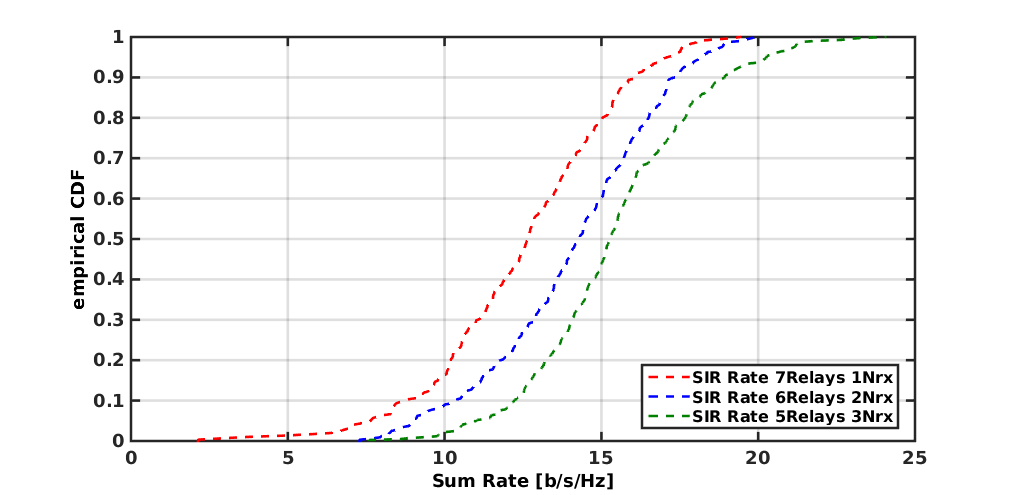
\includegraphics[width=0.9\linewidth]{images/ConstNrelNrx8comparison_1Rx_onlySIR.png}
\caption{Comparison of constant $N_\text{Rel} + N_{\text{Rx}} = 8$, with $N_\text{Rel}\in\{4,5,6,7\}$ and $N_{\text{Rx}}\in\{1,2,3,4\}$ from left to right, showing only noise free rates.}
\label{fig:1user_const_SIR}
\end{figure}
Therefore we can stick with a system, which uses one receiver antenna and multiple relays, and can expect to perform close to MIMO system with a sufficient large number of receive antennas to zero-force any interference.

Figure~\ref{fig:1user_const_SIR} shows the noise free, hence interference limited rates for a constant number of relays and receivers.
The SIR-rate for the receiver with four antennas is neglected, as the interference can be fully eliminated.
Again, it can be seen, that the larger the number of receive antennas, the better the interference can be reduced.
However, the differences are~---~as mentioned above~---~small.
Therefore we can conclude, that a system can almost perform the same by increasing the numbers of relays, as it would increasing the number of receive antennas.


\section{Four User System}
In the previous sections, the requirements for a system with three interferers were given.
Therefore in the following sections a full four user system will be analyzed and it will be shown, if the conclusions drawn from the previous sections were correct.

\subsection{Prediction for four Users}
\label{sec:const_prediction}
By the results shown in the previous section, the performance of a four user system can now be predicted.
A simulation of a four user system with widely spread receivers should lead to the same results like summing up the previous curves four times.
\begin{figure}[h]
\centering
  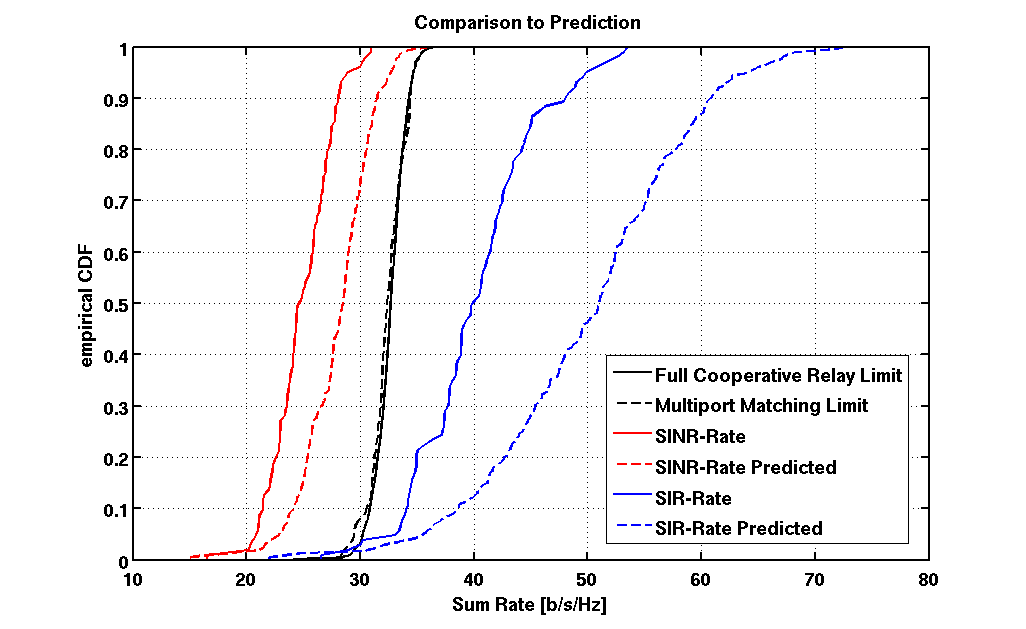
\includegraphics[width=\linewidth]{images/4user_inklpred.png}
\caption{Plot of the 4 User System, with the predicted performance.}
\label{fig:4user_pred}
\end{figure}

Figure~\ref{fig:4user_pred} shows the predicted performance (dashed lines) compared to the simulated performance (solid lines).
The rates of the simulated realizations are hereby lower than the predicted behavior.
For the simulation, the receivers were not place widely spaced apart, which is one reason for the lower rates, as the coupling among the receivers is diminishing the performance.
The second reason is, as mention above, a lower performance of the optimization algorithm with a larger problem.
Still we can conclude, that the optimal solution must be placed between the solid and the dashed curves.

Additionally, by the black curves, theoretical limits of the sum rates are given.
Because the predicted performance is not outperforming the theoretical limits, it consolidates, that the optimal solution lies around the predicted performance.


\begin{figure}[h]
\centering
  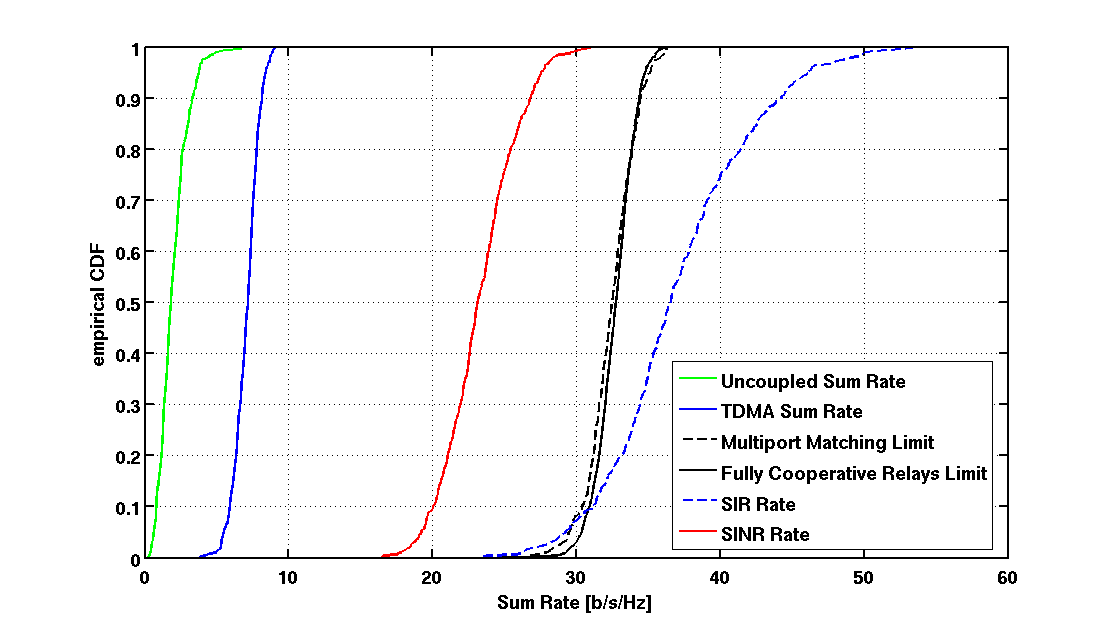
\includegraphics[width=\linewidth]{images/4user_sumrate.png}
\caption{Sum rates of a 4 user MIMO system.}
\label{fig:4user_sumrate}
\end{figure}
\subsection{Full Four User System Performance}
\label{sec:4user_const}

Finally we want to analyze the relay and matching network optimization of a four user system.
Two different realizations and antenna placings can be seen in Figure~\ref{fig:4user_placing}.
The achievable rates after optimization will be analyzed in the following for such placings.


Figure~\ref{fig:4user_sumrate} shows the sum rate of the optimized system (red solid curve) compared to the rates we introduced in the beginning of this chapter.
We see, that the uncoupled rate, i.e. each receiver has only one receive antenna and no relays, and the TDMA rate (under sum power constraint) are outperformed by far.
Further we see, that the noise free rate (dashed blue line) is always larger by  at least  $10 \left[\text{b/s/Hz}\right]$, which lets us conclude, that the interference cancellation was performed well, i.e. that we are in an interference free region for at least some users.
The black curves denoting the fully cooperative relays limit and the multi-port matching limit (dashed curve) are between $5 \left[\text{b/s/Hz}\right]$ and $10 \left[\text{b/s/Hz}\right]$ bits per second larger than the optimized sum rate.
From Figure~\ref{fig:relcomp_3} we know, that the limits are around $2 \left[\text{b/s/Hz}\right]$ larger than the optimized sum rate per user.
This shows, that at the median for four users, the optimization algorithm performs almost as good as for one user, however the lower rates seem to suffer from a bad optimization.

\paragraph{}
\begin{figure}[h]
\centering
  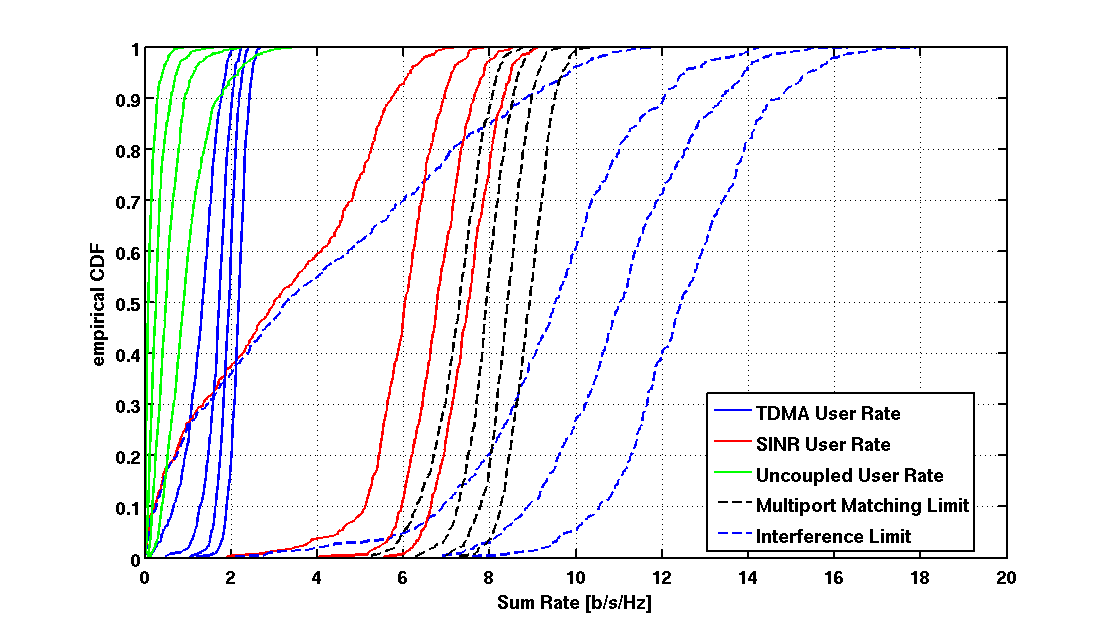
\includegraphics[width=\linewidth]{images/4user_userrate.png}
\caption{The user rates for  four users with seven relays each.}
\label{fig:4user_userrate}
\end{figure}
We saw in Figure~\ref{fig:relcomp_3} that it requires at least seven relays for one user to eliminate the interference from three users.
Figure~\ref{fig:4user_userrate} shows the rates for each transmit/receive pair by the red solid curves.
Again, the black dashed curves denote the multi-port matching rates, the green solid lines denote the performance if the relays were uncoupled, and the blue solid line shows the TDMA rate for each user under the sum power constraint.


We observe at first, that the uncoupled rate as well as the TDMA rate are outperformed by around $5 \left[\text{b/s/Hz}\right]$ for the three top users at the median.
The lowest user however is - contradicting to the results from Section~\ref{sec:3interf} - not interference free for almost 50\% of the cases.
For 10\% of the cases it even shows a worse performance than the TDMA rate.
It seems, that this user is for some realizations blocked, in order to enhance the other three users.
This might be the optimal solution, it might however also be, that the solver did not reach the best optimum.

To explore this a little bit further, Figure~\ref{fig:4user_placing} shows typical placings when the minimum user rate could be improved strongly on the left and when the rate could only be improved a little on the right.
Both subplots show a field of size $2\lambda \times 2\lambda$.
For the left subplot, the receivers have a larger distance between each other and the relay belongings to the receiver can be easy distinguished - they are more or less nicely separated.
This also accounts for receiver one and three in the subplot on the right, however receiver two and four are not so nicely separated anymore.
Additionally their distance is smaller than $0.5\lambda$.
This leads to a stronger coupling between the receiving elements of receiver two and four.
\begin{figure}[h]
\centering
  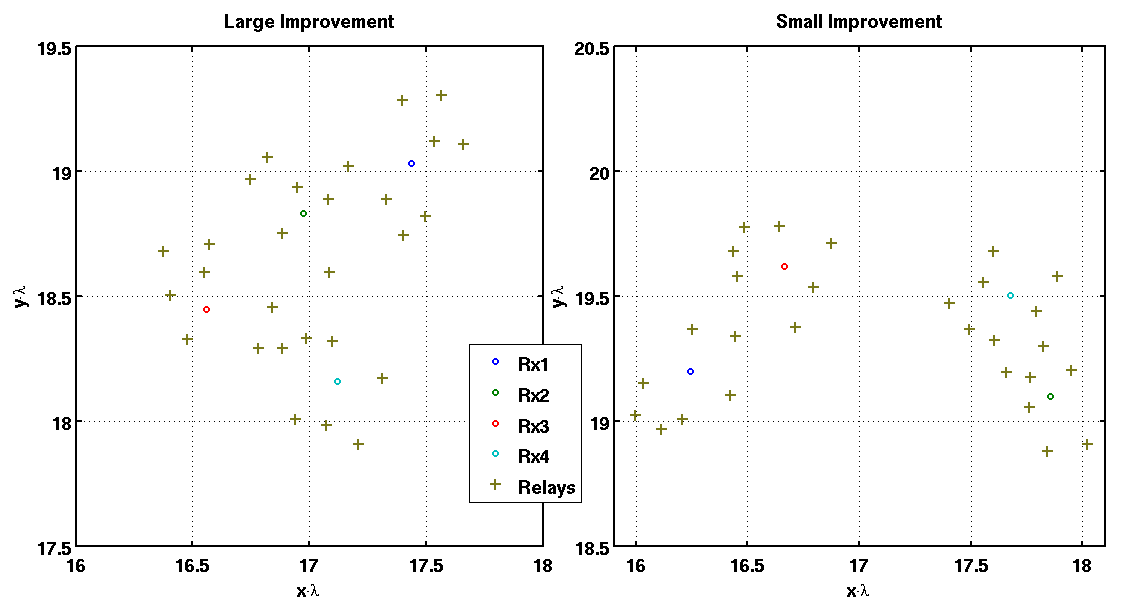
\includegraphics[width=0.8\linewidth]{images/Antenna_placing_4user.png}
\caption{Two different antenna placings, the left leads to a big improvement, the right to a small improvement.}
\label{fig:4user_placing}
\end{figure}

For the optimization this means, that if one receiver and its relays are optimized, their coupling might diminish the rate of the other receiver severely.
This effect can be seen as an additional interferer.
Any poor channel realization can lead than to a case, where the second receiver rate can not be optimized significantly anymore.


\section{TDMA - Combination}
\label{sec:tdma_combination}
In the following a combination of the optimization method with currently existing interference avoiding methods is analyzed.
As seen in the previous sections, the number of required relays, to reduce the interference grows with the number of users in the the system.
For large systems with hundrets of users the required number of relays hence would become extremly large.
Therefore a combination with the TDMA method is one way, to reduce the number of users in one time slot, hence it reduces the number of required relays.

Using two slot TDMA, reduces the number of users per slot from four to two.
Therefore, the results from Figure~\ref{fig:4user_sumrate} can be used to compare them to TDMA applied on the results from Figure~\ref{fig:iniopt_comp}.
The combination of TDMA and the optimization introduced in this thesis leads additionally to half the problem size, therefore results closer to the (corresponding) optimum can be expected from 2-slot TDMA, than from the pure optimization.
\begin{figure}[h]
\centering
  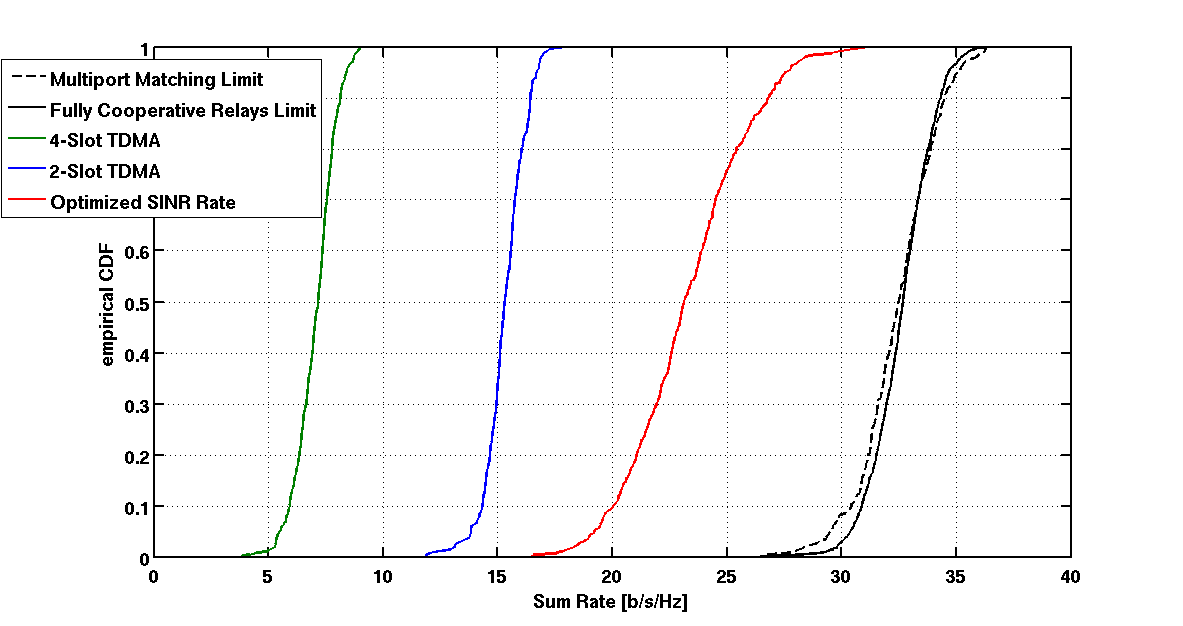
\includegraphics[width=\linewidth]{images/SlotTDMAcomparison_edited.png}
\caption{Comparison of different slot TDMA approaches.}
\label{fig:tdma_comb}
\end{figure}

Figure~\ref{fig:tdma_comb} shows in red the results of the four user system without TDMA (or 1-slot TDMA).
In blue the performance of the 2-slot TDMA approach applied on a four user system with only three relays per receiver is shown.
And in green the performance of a 4-slot TDMA approach without the use of any relay is shown.
Still the method introduced in this thesis without the use of TDMA outperforms 2- and 4-slot TDMA.
However it can also be observed, that the use of only three relays per user and a 2-slot TDMA approach outperforms the pure TDMA approach by approximately $8 \left[\text{b/s/Hz}\right]$.
Hence the combination of using passive relays and TDMA also significantly improves the performance of a system suffering from strong interference.

\begin{figure}[h]
\centering
  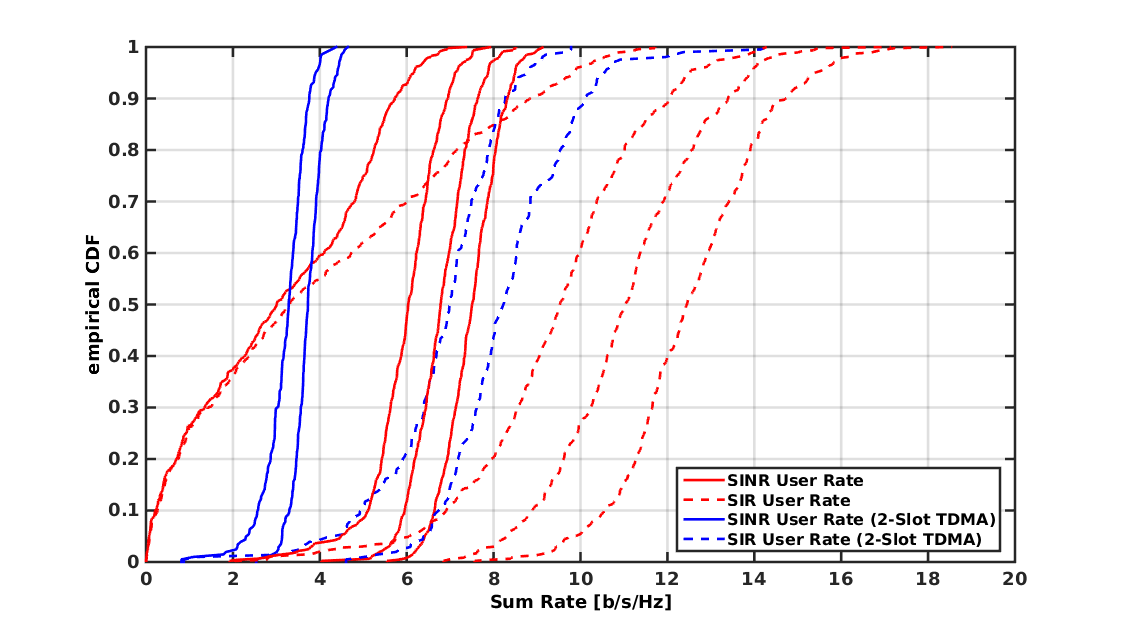
\includegraphics[width=\linewidth]{images/SlotTDMAcomparison_user.png}
\caption{Comparison of different slot TDMA approaches.}
\label{fig:tdma_comb}
\end{figure}





